\section{Essoufflement et froid}

\begin{frame}{Essoufflement}
  \begin{itemize}
    \item Comparable à l’essoufflement en course à pied.
    \item Effort trop important + mauvaise ventilation (surtout expiration).
    \item Augmentation du \textbf{CO\textsubscript{2}} $\Rightarrow$ sensation d’oppression, panique possible.
  \end{itemize}

  \begin{block}{Prévention}
    \begin{itemize}
      \item Avoir une \textbf{bonne condition physique}.
      \item Rester \textbf{calme} avant et pendant la plongée.
      \item Produire des \textbf{efforts modérés}.
      \item Ne pas être surlesté.
      \item \textbf{Forcer l’expiration} tout au long de la plongée.
    \end{itemize}
  \end{block}
\end{frame}

\begin{frame}{Reconnaître et signaler l’essoufflement}
  \begin{columns}[c]
    \begin{column}{0.6\textwidth}
      \begin{itemize}
        \item Ventilation \textbf{rapide et superficielle}.
        \item Sentiment de ne plus arriver à reprendre son souffle.
        \item Sentiment d’angoisse possible.
      \end{itemize}

      \begin{block}{Conduite à tenir}
        \begin{itemize}
          \item Faire le signe \og \textbf{je suis essoufflé} \fg{} au guide de palanquée.
          \item Réduire l’effort, se calmer, ventiler lentement et profondément.
        \end{itemize}
      \end{block}
    \end{column}
    \begin{column}{0.4\textwidth}
      \centering
      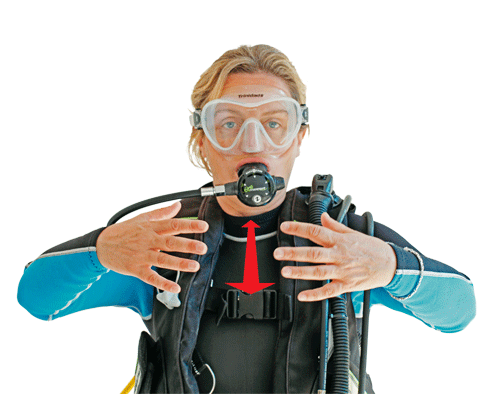
\includegraphics[height=0.5\textheight]{images/signes_essoufflement-2}
    \end{column}
  \end{columns}
\end{frame}

\begin{frame}{Le froid}
  \begin{columns}[c]
    \begin{column}{0.6\textwidth}
      \begin{itemize}
        \item Dans l’eau, le corps se refroidit \textbf{25 fois plus vite} qu’à l’air libre.
        \item Combinaison inadaptée : trop large $\Rightarrow$ circulation d’eau ; trop serrée $\Rightarrow$ gêne la ventilation.
      \end{itemize}
    \end{column}
    \begin{column}{0.4\textwidth}
      \centering
      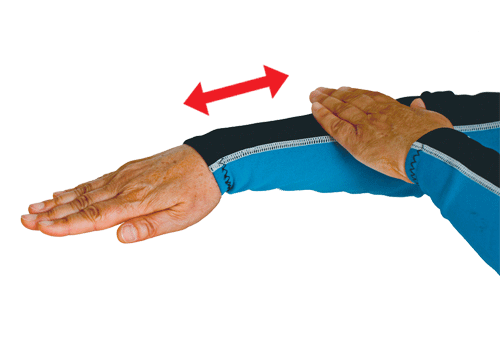
\includegraphics[height=0.4\textheight]{images/signes_froid-2}
    \end{column}
  \end{columns}
  \begin{block}{Prévention}
    \begin{itemize}
      \item Combinaison adaptée à la \textbf{température de l’eau} et à la morphologie.
      \item Alimentation avec \textbf{sucres lents} (repas) et \textbf{sucres rapides} avant la plongée.
      \item Pas d’alcool, éviter de plonger fatigué.
      \item Se couvrir avant et après la plongée.
      \item Signaler le froid : signe \og \textbf{j’ai froid} \fg{}.
    \end{itemize}
  \end{block}
\end{frame}
